
%% manuscript produces a one-column, double-spaced document:
\documentclass[12pt,a4paper,twoside]{report}
%\documentclass[12pt, manuscript]%{aastex}
%\usepackage{graphicx}
%\usepackage[utf8]{inputenc}
%\usepackage[ipaex]{pxchfon}
\usepackage{graphicx}
\usepackage{amsmath,amssymb,amsfonts}
\usepackage{subfig}
\usepackage{natbib, aas_macros}
\citestyle{aa}
\usepackage{setspace}
\usepackage{times}
\usepackage{rotating}
 \usepackage{fancyhdr}
\usepackage{booktabs}
\usepackage{gensymb}
\usepackage{lineno}
\usepackage{footnote}
\usepackage{tablefootnote}
\usepackage{url}
\usepackage{CJKutf8}

%%% packages for pretty timeline %%%
%\usepackage[utf8]{inputenc}
%\usepackage[TS1,T1]{fontenc}
%\usepackage{fourier, heuristica}
\usepackage{array}
%\usepackage{graphicx}
\usepackage[x11names]{xcolor}
\usepackage{colortbl}
\usepackage{caption}
\usepackage{listings}
\usepackage{lmodern}
\usepackage[T1]{fontenc}
\newcommand{\foo}{\makebox[0pt]{\textbullet}\hskip-0.5pt\vrule width 1pt\hspace{\labelsep}}

%%%

%%%%%%%%%%%%%%%%text size and spacing%%%%%%
%%% Number equations according to section %%%
\numberwithin{equation}{section}

%%% text size %%%
\setlength{\topmargin}{10mm}
\addtolength{\topmargin}{-1in}
\setlength{\textheight}{262mm}
\setlength{\headsep}{5mm}
\setlength{\headheight}{0mm}
\setlength{\topskip}{0mm}
\setlength{\oddsidemargin}{-1in} %  set real left margin 0pt
\setlength{\evensidemargin}{-1in} % do
\addtolength{\oddsidemargin}{25mm} % odd page 25mm left margin
\addtolength{\evensidemargin}{15mm}% even page 15mm left margin
\setlength{\textwidth}{170mm}
%\setlength{\leftmargin}{-1 in}

\pagestyle{fancy}
\lhead[\it\scriptsize \leftmark]{}
\chead[]{}
\rhead[]{\it \scriptsize \rightmark}
\renewcommand{\headrulewidth}{0.4pt}
\renewcommand{\footrulewidth}{0pt}
\renewcommand{\baselinestretch}{1.}
\renewcommand{\bibname}{References}

\doublespacing

\title{AKARI and Spinning Dust Emission\\
A look at microwave dust emission via the Infrared\\
\begin{CJK}{UTF8}{min}\LARGE{\bf あかりで探るスピニングダスト:\\
赤外で見たマイクロ波ダスト放射}\end{CJK}
Doctoral Thesis\\
Submitted to The University of Tokyo\\
DRAFT}

\author{Aaron Christopher Bell}

\begin{document}
\maketitle

\pagenumbering{roman}
\linenumbers
\makesavenoteenv{tabular}
\makesavenoteenv{table}

\singlespacing
\tableofcontents
{\small \listoffigures}

\doublespacing
\chapter*{Abstract}
\addcontentsline{toc}{chapter}{Abstract}
The anomalous microwave emission (AME) still lacks a conclusive explanation.  This excess of emission, roughly between 10 and 50~GHz, tends to defy attempts to explain it as synchrotron or free-free emission. The overlap with frequencies important for cosmic microwae background explorations, combined with a strong correlation with interstellar dust, drive cross-disciplinary collaboration between interstellar medium and obervational cosmology. The apparent relationship with dust has prompted a ``spinning dust'' hypothesis:  electric dipole emission by rapidly rotating, small dust grains. Magnetic dipole emission by grains with magnetic inclusions (``magnetic dust''), while less suppported, has not been ruled out. Even assuming a spinning dust scenario, we are far from concluding which category of dust contributes. The typical peak frequency range of the AME profile implicates grains on the order of ~1nm. This points to polycyclic aromatic hydrocarbon molecules (PAHs). We use data from the AKARI/Infrared Camera (IRC; \citet{irc07}), due to its thorough PAH-band coverage, to compare AME from the \cite{planck15X}. astrophysical component separation product) with infrared dust emission. We look also at infrared dust emission from other mid IR and far-IR bands. The results and discussion contained here apply to an angular scale of approximately 1$^{\circ}$. In general, our results support an AME-from-dust hypothesis. We look both at $\lambda$~Orionis, a region highlighted for strong AME, and find that certainly dust mass correlates with AME, and that PAH-related emission in the AKARI/IRC 9~$\mu$m band may correlate slightly more strongly. These results are compared to an all-sky analysis, where we find that potential microwave emission component separation imperfections among other issues, make an all-sky, delocalized comparsion very challenging. In any case the AME-to-dust correlation persists even in the all-sky case, but tests of relative variations from different dust SED components are largely inconclusive. We emphasize that future efforts to understand AME should focus on individual regions, and a detailed comparsion of the PAH features with the variation of the AME SED. Further all-sky analyses seem unlikely to help resolve this issue. Non-PAH carriers of the AME, such as nanosilicates, cannot be ruled out either.

\pagenumbering{arabic}
All-sky astronomy is not new. Indeed, the notion of capturing a particular "object" or "source" with a camera and saving it for later investigation would be completely alien to the first astronomers and astronavigators. Absence of telescopes forced us to describe the sky in terms of its larger patterns, brightest characters. What is new however, is the notion of preparing an archive of the sky itself for not only the research whims of a single investigator, team, institute, or even a single nation- rather, all-sky surveys tend to be international endeavors in their production, and even more so in their utilization.

This is especially true in the context of infrared astronomy, a field which was essentially non-existant as recently as the 1950s \citep{johnson66} \footnote{1920s, if we judge by the first IR observations}. Compare this to visible wavelength- a field so old we name it after the bio-evolutionary advent of sight, itself. Even radio astronomy with its own logistical and technological challenges, has been around since at least 1932.

`` Johnson+ 1966 p.194: "It is now plain that about 75\% of the data we would like to have can be obtained from good ground-based sites"
% ...p.1 "The Far Infrared, from 4 to 22 um''

Despite the above claim from \citep{johnson66}, astronomers were apprently not content to be constrained by atmospheric IR windows, even from the best of ground-based sites. Or perhaps interests have shifted so dramtically since 1966, that all of the investigations enabled by rocket-based, space-based, even Boeing 747-based IR astronomy would have bored 75\% of astronomers in the '60s.

\chapter{Data Sources}
  \label{ch:datasources}

  \section{A collection of skies}
    This work relies completely on all-sky surveys. All of the maps utilized are photometric-band infrared maps, except for the AME data, which is an all-sky component separation analysis product, from the Planck Collaboration's efforts to separate galactic foregrounds from the CMB.


    \begin{table}[h]
      \label{tab:data}
      \caption{Observational data sources used in this article}
      \centering
        \begin{tabular}{lrrrrr}
        \hline\hline
        Instrument & Central Wavelength & FWHM & Cali & Reference \\
        \hline
        AKARI/IRC & 9~$\mu$m  &  \~{}10$"$ & \textless 10\%   & \tablefootnote{\citep{ishihara10}} \\
        AKARI/IRC & 18~$\mu$m & \~{}10$"$  & \textless 10\%     & '' \\
        AKARI/FIS & 65~$\mu$m  & 63$"$ & \textless 10\% & \tablefootnote{\cite{doi15,takita16}} \\
        AKARI/FIS & 90~$\mu$m  & 78$"$ & \textless 10\%   & '' \\
        AKARI/FIS & 140~$\mu$m & 88$"$ & \textless 10\%   & '' \\
        AKARI/FIS & 160~$\mu$m & 88$"$ & \textless 10\%   & '' \\
        IRAS/IRIS & 12~$\mu$m   & 4.0$'$ &   \textless 5.1\%       & \tablefootnote{\cite{iris05}} \\
        IRAS/IRIS & 25~$\mu$m   & 4.0$'$ &    \textless 15.1\%      & ''\\
        IRAS/IRIS & 60~$\mu$m   & 4.2$'$ &    \textless 10.4\%      & '' \\
        IRAS/IRIS & 100~$\mu$m  & 4.5$'$ &   \textless 13.5\%       & '' \\
        Planck/HFI & 345~$\mu$m & 4.7$'$ & & \tablefootnote{\cite{hfi14viii}} \\
        Planck/HFI & 550~$\mu$m & 4.3$'$& & '' \\
        \hline
      \end{tabular}
    \end{table}

  \subsection{Primary band of interest}\footnote{Not to be confused with ``The band primarily interested'' in dust, Queen.}
    The AKARI/IRC 9~$\mu$m band (A9) provides uniquely complete coverage of the PAH bands at 6.2, 7.7, 8.6, and 11.2~$\mu$m, and may be an excellent tool for testing PAH-related hyoptheses on an all-sky basis. The combination of A9 with W12 and/or I12 may be especially insightful. In total, we employ all-sky maps from 12 photometric bands, spanning the wavelength range of 6.9~$\mu$m to 550~$\mu$m\footnote{Planck bands are named according to their central frequency, not wavelength.}

  \section{Infrared Data}
    \subsection{AKARI}
       The AKARI infrared space telescope revealed an entire sky of infrared light, from the mid to far infrared, via two instruments \citep{akari07} the Infrared Camera (IRC)\citep{irc07} and the Far Infrared Surveyor (FIS) \citep{fis07}.

       \paragraph{AKARI/IRC PAH feature coverage}
         The IRC's 9~$\mu$m band all-sky map demonstrates the abundance of the PAH bands carrier in the Milky Way \citep{ishihara10}. Figure \ref{fig:relSpectralResponse_MIR} shows the coverage of the MIR bands along with an example galactic cirrus SED. The 9~$\mu$m band uniquely covers major ionized PAH features at 6.2 and 7.7~$\mu$m; as well as neutral PAH features at 8.6 and 11.2~$\mu$m across the entire sky \citep{irc07}. The IRAS 12~$\mu$m band covers the 11.2 and 8.6~$\mu$m features, and the similarly-shaped WISE~12~$\mu$m band covers primarily the 11.2~$\mu$m feature.

         \paragraph{In-band conribution from PAHs}
           According to this distribution of PAH features across the response filters, it is expected that the IRC 9~$\mu{}$m band is most dominated by PAH emission even with increasing $G_0$. These contributions remain relatively constant out to a $G_{0}$ of about 100, with the contribution from warm dust becomming a larger factor for the IRAS 12~$\mu$m and WISE 12~$\mu$m bands. Thus, according the the DL01 template, IRC 9~$\mu$m should have the highest contribution from PAHs out to extreme radiation fields.

          \paragraph{Potential to trace PAH ionization}
            Fig. \ref{fig:inband_ionfrac_ratios} demonstrates how the band ratios of the IRC 9um band vs. the other MIR bands change with different modeled PAH ionization fractions (determined using the DustEM default model template, by \cite{dustem11}. This band ratio can be determined, because the IRC9 filter is more sensitive to ionized PAH features, relative to IRAS12 or to WISE12.
           IRC 9~$\mu$m shows a larger contribution from ionized PAHs, by about 16 percent, and a conversely smaller contribution from neutral PAHs.

       \begin{figure*}
       \label{fig:relSpectralResponse_MIR}
       \centering
       \includegraphics[width=150mm]{../Plots/RelSpectralResponse_MIR.png}
       \caption{Relative spectral response curves of the MIR bands used in this study, AKARI/IRC 9~$\mu$m, IRAS 12~$\mu$m, WISE 12~$\mu$m, AKARI 18~$\mu$m, and  IRAS 25~$\mu$m. AKARI/IRC 9~$\mu$m, IRAS 12~$\mu$m, WISE 12~$\mu$m bands are dominated by PAH emission.}
       \end{figure*}


       \begin{figure*}
       \label{fig:inband_ionfrac_ratios}
       \centering
       \includegraphics[width=150mm]{../Plots/band-ratio-multiple.pdf}
       \caption{Ionization fraction of PAHs vs. band ratios of IRAS12 and 25, and WISE 12 and 25~$\mu$m bads vs. the AKARI 9~$\mu$m band, for three ISRF strengths: Top: $G_{0} = 100$, Middle: $G_{0} = 1000$, and Bottom: $G_{0} = 10000$. These ratios are determined by assuming the SED template if \cite{dustem11} }
       \end{figure*}

        We utilize the most recent version of the IRC data (Ishihara, et al., in prep.) This version has had an updated model of the Zodiacal light, fitted and subtracted. The details of the improved Zodi-model, which offers an improvement over that used for the IRAS all-sky maps, are given in \cite{kondo16}.



      The AKARI Far Infrared Surveyor (FIS) gives us photometric data around the peak of the typical thermal dust SED. FIS was equipped with four wavebands: two narrow bands centered at 65~$\mu$m and at 160~$\mu$m, and two wide bands at 90~$\mu$m and at 140~$\mu$m. An all-sky survey was carried out at each band \citep{kawada07}, and the processed maps have been publicly released \citep{doi15}.

       The Planck Space Observatory (Planck) High Frequency Instrument (HFI) all-sky maps, spanning 100 to 857~GHz \citep{hfi14viii} help constrain the far IR dust emissivity. This study utilizes the 857~GHz (345~$\mu$m) and 545~GHz (550~$\mu$m) bands.

       Data from the Infrared Astronomical Satellite \citep{iras84} all-sky surveys are used to supplement the similarly-centered AKARI photometric bands. The IRAS 12~$\mu$m band is similar to the AKARI 9~$\mu$m band in terms of the sky coverage, central wavelength, and especially in that both surveys are heavily dominated by zodiacal light. We use the Improved Reprocessing of the IRAS Surveys (IRIS) \citep{iris05}, which use undergone a zodiacal-light removal. The Zodiacal light model, however differs between the two bands. The IRAS Zodi-subtraction is primarily based on the \cite{kelsall98} model.

  \section{Planck COMMANDERAME Parameter Maps}

       We utilize the COMMANDER-Ruler astrophysical component separation maps, from the Planck Collaboration's Public Data Release 2 (hereafter, PR2). These contain estimates of known microwave foreground components (free-free, synchrotron, thermal dust emission contributions to the Planck photometric bands. Details of the foreground contribution estimates are given in \cite{planckXII}. We will first describe the 'non-AME' components, so as to not give any indiciation that their estimation is trival.

       \begin{figure*}
         \label{fig:PCCS_corrmatrix}
         \includegraphics[width=\textwidth]{../Plots/ch_datasources/PCCS_corrmatrix.pdf}
         \centering
         \caption{All-sky map of the peak frequencies of the varying component $AME_{var}$, corresponding to Fig. \ref{fig:AME_commander_freqdist}.}
       \end{figure*}

       \subsection{Synchrotron}
        While the Planck observations themselves do limit our resolution when assessing the AME - it is in fact the primary constraint on synchrotron emission, 408~MHz map by \cite{haslam82} that is the major resolution limiting factor. While an impressive, pioneering effort for to reveal the low-frequency sky, \citep{haslam82} is limited to an appriximately 1 degree resolution. The map also contains
        many artifacts. For the time being however, it is still the most synchrotron-dominated all-sky map available, and for this reason PC15X included it in their COMMANDER component separation. The final synchrotron product produced by COMMANDER (hereafter, PCSync) highly resembles the \citep{haslam82} map, however it is also demonstrated PCSync does not fully capture the synchrotron signal. This can be visualized by inspecting the PCAME:PCdust ratio map (see Fig. \ref{fig:R_PCAMEtoPCdust}), which \cite{hensley17} describe as containing synchrotron emission patterns at high latitudes.

        \begin{figure*}
        \label{fig:R_PCAMEtoPCdust}
        \centering
        \includegraphics[width=\textwidth]{../Plots/ch_datasources/R_PCAMEtoPCRad.pdf}
        \caption{All-sky map of the ratio of two COMMANDER components- the frequency-varying AME component divided by the intensity of thermal dust emission at 545~GHz. }
        \end{figure*}

       \subsubsection{Free-free emission}
        Unlike the PCSync component, the fitting of the Planck COMMANDER free-free component map (hereafter, PCff) does not employ any free-free dominated emisison map.\footnote{The Planck AME paper, \cite{planckXV}, had employed the H-$\alpha$ map by \cite{wham98}}.

      \subsection{Thermal dust emission}

      ``Thermal dust emission'' in the COMMANDER context refers to dust emission in the Rayleigh Jeans-regime, as the COMMANDER fitting does not include photometric constraints on the thermal emission peak, or consider small grain emission on the Wiens side.

       \subsection{COMMANDER-AME: Peak Frequency Distribution}

        $I_{AME}\nu_{var}$
        In addition, there is an ``AME component map'', which presumes that AME originates from spinning dust. While acknowledging that such a decomposition lacks a physical justfication, \cite{planck15X} break the AME into two components: a spatially varying peak frequency component, and a spatially constant peak frequency component. However as seen in Fig. \ref{fig:AME_commander_freqdist}, virtually all of the fitted peak frequncies for $AME_{var}$ beyond the reach of WMAP and Planck. Only the fitted global frequency, 33.5~GHz for the spatially constant component, is covered.


        \begin{figure*}
          \label{fig:AME_commander_freqdist}
          \includegraphics[width=\textwidth]{../Plots/ch_intro/AME_commander_freqdist.pdf}
          \centering
          \caption{The peak frequencies of the varying component $AME_{var}$.  The pink shaded region indicates frequencies not covered by either WMAP or Planck The green line at 33.5~GHz indicates the peak frequency of $AME_{fix}$.}
        \end{figure*}

        \begin{figure*}
          \label{fig:PCAME_var_freq.pdf}
          \includegraphics[width=\textwidth]{../Plots/ch_datasources/PCAME_var_freq.pdf}
          \centering
          \caption{All-sky map of the peak frequencies of the varying component $AME_{var}$, corresponding to Fig. \ref{fig:AME_commander_freqdist}.}
        \end{figure*}

        %The next figure shows the all-sky ratio map, of $AME_{var}:AME_{fix}$. That is, the ratio of the integrated intensities of these components, rather than the intensities given directly in the COMMANDER maps.
        The COMMANDER maps give each component's intensity at a different ``reference frequency'' (corresponding to photometric bands). In other words, the COMMANDER AME intensities are not peak intensities. Moreover they are intensities calculated for a single template spinning dust spectrum- but one that has been log-log translated to fit the observations (a demonstration of such shifted templates, for a common ``reference intensity'' at a common ``reference frequency'', is shown in Fig. \ref{fig:AME_commander_freqshift_templ}). The physical paraneters in the spinning dust model, ``spdust'' are not varied.

        \begin{figure*}
          \label{fig:AME_commander_freqshift_templ}
          \includegraphics[width=\textwidth]{../Plots/ch_datasources/AME_commander_freqshift_templ.pdf}
          \centering
          \caption{Spdust template spinning dust profiles fitted by PC15 when calculating $AME_{var}$.  The reference frequency, 22.8~GHz is indicated by the vertical green line. Each template has the same $AME_{var}$ amplitude of 100~$\mu$K, indicated by the horizontal green line, plotted to highlight the potential deviation between $AME_{var}$ and the actual peak intensity. }
        \end{figure*}

        For these reasons, we are very cautious in deriving conclusions from comparisons with the COMMANDE AME map. Indeed, the authors themselves include a similar disclaimer. However since there is currently no better all-sky component separation available\footnote{Indeed, improving on the COMMANDER AME map would be extremely difficult without lower frequency constraints and/or higher resolution observations of not only the AME itself but the contribution from synchrotron and free-free emisson.}, and carrying out a spinning dust modeling and component separation is beyond the scope of this work, we proceed with care.


  \section{All-sky Data Processing}

        The HFI, FIS, and IRIS maps used here are downloaded from their respective online repositories, as all-sky HEALPix\footnote{HEALPix core software is described at \url{http://healpix.sourceforge.net}. The HEALPIx python package ``healpy'' used in this work is available at: \url{https://github.com/healpy/healpy}} maps \citep{gorski05}.   NSIDE 2048 maps. In the case of the IRC maps, we first create HEALPix maps from the 4,857 all-sky survey tiles using the Aladin all-sky data visualization platform \citep{bonnarel00}. NSIDE 2048 implies an average pixel spacing of 1.7$'$. The maps are then degraded to NSIDE 1024 before carrying out a Gaussian-beam smoothing to a 1$^{\circ}$ FWHM \footnote{To be clear, maps are converted first to spherical harmonic space, smoothed, and transformed back to position space using - steps carried about by the smoothing function contained in the healpy python package}. Following the smoothing process, the maps are degraded once more to NSIDE 256, or 15arcmin pixel-width \footnote{HEALPix pixel scale rebinning carried out with healpy.ud\_grade}. The value of each of the larger NSIDE 256 pixels, comes from the mean of its parent NSIDE 1024 pixels. The purpose of this processing is to ensure that all of the maps have the same resolution as the PR2 AME map.

\chapter{Analysis of an interesting \acrshort{ame} region: $\lambda$~Orionis}
\label{ch:lori}
  This chapter is an analysis of the \acrshort{ame} and how it relates to the dust emisison, in the $\lambda$~Orionis region. This has been an ongoing collaboration with F. Galliano, an expert in dust \acrshort{sed} fitting and developer of a dust \acrshort{sed} framework presented in \cite{galliano18}. This work has been enabled by mutual collaboration vists by myself and F. Galliano, funded in part by a joint JSPS-CNRS international collaboration grant. The results described here are intended to form the core of a journal publication, to be submitted in the coming months.

 \section{An interesting \acrshort{ame} region}
		The $\lambda$~Orionis molecular ring, also known as the Meissa Ring is a massive stucture surrounding the $\lambda$~Orionis O-type star. The ring contains an HII region, ionized by $\lambda$Ori itself and its OB associates \citep{murdin77}. What had been thought of as a star\-forming region of missing molecular gas. At the time \cite{murdin77} even speculated that this could be evidence of an alternate star\-formation pathway, writing: ``Notably we need to know if $\lambda$Ori is an example of a different mode of star formation or [...] simply a case in which the progenitor molecular cloud was exhausted within the last one or two million years.''

    \cite{maddalena86,maddalena87}.  (and references therein) noted a ring of material likely being pushed out by the central, historically well-known $\lambda$~Orionis Association of B-type stars and surrounding HII reigon.


    \cite{cunha96} argued that the ring shape around $\lambda$~Orionis may have resulted from a supernova explosion, further speculating that $\lambda$Ori may have been a companion of the progenitor. $\lambda$~Orionis is a known binary system, however its current companion is a B-type star. \citep{murdin77}
  .
     The central region is heated by the $\lambda$~Orionis star itself, and the Orion~OB association it belongs to \citep{ochsendorf15}. The region is known to host several young stellar and protostellar objects \citep{koenig15}.

    At approx. 10$^{\circ}$ wide, we can see the outline of the structure even in the low (1$^{\circ}$ FWHM) resolution PCAME map. The ring shape itself is thought to originate from a supernova, or perhaps combined effects of the entire star formation history of the $\lambda$~Orionis Association, including the formation of its surrounding HII region \citep{aran09}.

    Although the $\lambda$~Orionis region has been a popular target for study since approximately the 1980s. \cite{duerr82} wrote of the relative lack of work on the overall region: ``Surprisingly, this interesting complex has been little studied''. While this seems surprising given the numbe of works on the region in the literature now, it is really the advent of all-sky missions that have driven more recent interest.  The large angular size is such that all-sky surveys were a natural boon for study of such extended structures. WISE especially was a huge source of insight \citep{koenig15}. More recently, \cite{planck15XXV} strongly highlighted the region as a strong candidate for further \acrshort{ame} investigation.

\section{Investigative approach}
  We have carried out an initial comparison of the \acrshort{ame} of this region with its mid to far-IR dust emission. The region is shown in Fig.~\ref{fig:orionis-akari9} as it appears in 1$^{\circ}$-smoothed A9 data.
      \begin{figure}
        \includegraphics[width=\textwidth]{../Plots/LOri_akari9_AMEcont_1dres.pdf}
        \centering
        \caption{$\lambda$~Orionis as it appears in the AKARI 9~$\mu$m data. Contours indicate the \acrshort{ame}, as given by the Planck PR2 \acrshort{ame} map. The image is smoothed to a 1$^{\circ}$ PSF (much larger than the original 10 arcsec map). The $\lambda$~Orionis star itself is approximately located at the center of the image.}
        \label{fig:orionis-akari9}
      \end{figure}
   The ring structure itself indicates excess microwave emission attributed to \acrshort{ame}, from the dominant variable frequency component $AME_{var}$ (see Ch.~\ref{ch:datasources}). The central region is dominated by free-free emission \citep{aran09, koenig15}. Free-free emisison coming from the Hii phase surrounding the $\lambda$~Orionis association dominates the region's morphology in \acrshort{lfi} images. \citep{planck15XXV}. Taking the hint from \cite{planck15XXV} that this may be among the more reliably component separated regions, we evaluate if there is any preferential relationship between any parameter of dust emission and the \acrshort{ame}. Fig.~\ref{fig:LOri_halpha_AMEvarContours} shows the expected distribution of free-free emission in the region, assuming that $H\alpha$ line emission is a tracer of microwave free-free. This indicates that free-free is strong within the central region, where radiation fields are more intense, and \acrshort{ame} is minimal. The strongest \acrshort{ame} follows the ring-shaped morphology outside the central bubble of free-free emission.
     \begin{figure}
       \includegraphics[width=\textwidth]{../Plots/ch_lori/LOri_halpha_AMEvarContours.pdf}
       \centering
       \caption{$\lambda$~Orionis as it appears in H-alpha emission by \cite{finkbeiner03}. Contours indicate \acrshort{ame} emission, from the variable frequency component. The colorbar indicates $H\alpha$ emission in Rayleighs. The field of view is slightly larger than that used for the final processed IR comparison (Fig.~\ref{fig:lori_processed_all}). }
       \label{fig:LOri_halpha_AMEvarContours}
     \end{figure}
    We will first show a model-independent analysis, comparing IR photometric intensities from the mid to far-IR to the \acrshort{ame}. After comparing all of these intensities, we describe which wavelength shows the best intensity correlation. The core results however will be based on a dust SED model-dependent analysis, which takes into consideration all of the photometric intensities to fit the total abundance of dust, PAH abundance, PAH ionization fraction, and ISRF strength, $U$, accross the $\lambda$~Orionis region. We will then discuss the core result, suggesting that PAH mass has a stronger relationship with AME than the total dust mass does, representing the first time such a result has been found for a specific \acrshort{ame}-prominent region.

	\section{Data preparation}
    \label{sec:dataprocessing}
		As indicated in Ch.~\ref{ch:datasources}, we use 12 photometric all-sky maps. For the IRC data (A9 and A18), we produce mosiacs of $\lambda$~Orionis from the latest version of the individual tiles provided internal all-sky archive. A9 and A18 images are produced by regridding the images with the {\tt Montage} software by \acrshort{nasa}/\acrshort{ipac}. Figs.~\ref{fig:lori_A9_mosaic_smooth} and~\ref{fig:lori_A18_mosaic_smooth} show high resolution mosaics of the A9 and A18 data before processing.
      \footnote{IRC all-sky data is still in the proprietary phase at the time of this writing, but should be public by April 2018.}
       For the other sources, HEALPix all-sky maps are available publicly, at sufficient resolution relative to their native resolutions\footnote{Planck data was retreived from the NASA IPAC online archive at \url{http://irsa.ipac.caltech.edu/data/Planck/release_2/all-sky-maps/}}. \footnote{AKARI/FIS data }\footnote{IRAS/IRIS data }

		  Other data were obtained from publically archived HEALPix maps. This includes data from \acrshort{iras}, Planck, \acrshort{dirbe}, and AKARI/FIS. For For these data, we employ the {\tt healpix2wcs} functionality provided in the {\tt gnomdrizz} python package\footnote{Available at \url{http://cade.irap.omp.eu/dokuwiki/doku.php?id=software}}\footnote{``drizzlib'' 1.2.2 and earlier were not able to correctly access HEALPix files with multiple fields/columns. See appendix for our recommended workaround.}   When the extraction and regridding are finished, all of the images --- those extracted from \acrshort{healpix} maps, as well as the \acrshort{irc} data --- share a common FITS header having a pixel grid spacing equal to the average pixel width in the NSIDE 256 \acrshort{healpix} scheme, or about \textasciitilde{0.25$^{\circ{}}$}. After PSF smoothing, described in detail below, the data also have a common \textasciitilde{1$^{\circ{}}$} FWHM effective PSF. Although this means that the grid is oversampled, we choose this approach to preserve as much of the structure of the region as possible, even after masking bad pixels. Another option would be to interpolate the bad pixels, and degrade the pixel scale to the PSF size. However we choose the former method due to the relative large number of bad pixels, especially around the regions affected by missing stripes. This means that in the analyses that follow, what is important is the relative trends between correlation coefficients, rather than their absolute values.

      \subsection{Point-source and artifact masking}

        \paragraph{Missing stripes}
          The AKARI all-sky survey suffers from a few missing stripe errors throughout the \acrshort{irc} and \acrshort{fis} maps \citep{ishihara10, doi15}. This is a more serious issue for \acrshort{fis}. Unfortunately for the present work, some of these stripes pass directly through the $\lambda$~Orionis region. Figs.~\ref{fig:LOri_FIS_color},~\ref{fig:lori_A9_mosaic_smooth} and ~\ref{fig:lori_A18_mosaic_smooth} display the data at near-native resolution, demonstrating where these patterns occur. Additionally there are some saturated pixels in both \acrshort{irc} and \acrshort{fis} data.
            \begin{figure}
              \includegraphics[width=\textwidth]{../Plots/ch_lori/lori_fis_rgb.pdf}
              \centering
              \caption{The $\lambda$~Orionis region and its surroundings in AKARI \acrshort{fis} data, where A65 is blue, A90 is green, and A140 is red. The missing stripe patterns are visible, and affect all 3 bands shown here as well as the A160 data. }
              \label{fig:LOri_FIS_color}
            \end{figure}
            \begin{figure}
              \includegraphics[width=\textwidth,trim={2.5cm 2cm 3.0cm 2cm},clip]{../Plots/ch_lori/lori_A9_mosaic_smooth.pdf}
              \centering
              \caption{The $\lambda$~Orionis region in the A9 band at near-native resolution. This is a mosiac created from the 3x3 degree all-sky survey tiles by Ishirara et al. (in prep.) Missing stripes are less of a problem than with the A18 band (Fig.~\ref{fig:lori_A18_mosaic_smooth}), but point sources are more pronounced. Around Betelgeuse, in the lower left of the image, we can see an artifact caused by scattered light.. }
              \label{fig:lori_A9_mosaic_smooth}
            \end{figure}
            \begin{figure}
              \includegraphics[width=\textwidth,trim={2.5cm 2cm 3.0cm 2cm},clip]{../Plots/ch_lori/lori_A18_mosaic_smooth.pdf}
              \centering
              \caption{The $\lambda$~Orionis region in the A18 band at near-native resolution, demonstrating the regions affected by missing stripe errors, but less affected by point-sources than A9 (Fig.~\ref{fig:lori_A9_mosaic_smooth}). }
              \label{fig:lori_A18_mosaic_smooth}
            \end{figure}

        \paragraph{Point sources}
          A caveat that comes with added ionized \acrshort{pah} feature coverage of the A9 band, is that the shorter central wavelength placement allows more contamination from point sources. We identify point sources with a moving-window approach provided in the astropy Python package, flagging pixels which have higher than 5$\sigma$ intensity among the surrounding 100 pixel window. We then place a mask at the center of the flagged point-sources. The masks are propogated through the regridding step, such that the low-resolution pixels having more than 50\% of their area masked in the high resolution tiles, also become masked. Such pixels appear black in Fig.~\ref{fig:orionis-akari9}. The same process is applied to the A18 data. For other maps, which we extract from HEALPix data, we first regrid from \acrshort{healpix} to rectangular grids, and then apply the point-source search and masking as above. For the I12 and I25 images, the rejected pixels were fewer than with A9, but positions overlapped with those already masked in A9. For bands longer than I25, this process did not result in rejected pixels. For the D12 and D25 bands, which are natively at a much lower resolution than AKARI or \acrshort{dirbe}, point-sources present more of a challenge. For these images, we visually inspect and mask 3 regions with bright point source contamination consistent with the \acrshort{dirbe} beamsize and with point-sources identified in IRAS and IRC images. Pixel positions masked in any single image, are masked in all of the images before the finaly analysis.


        \subsection{PSF Smoothing}
          We smooth the pixels in the spatial domain, to have a 1$^{\circ}$ FWHM PSF, in order to have a resolution approximating that of the \acrshort{pc} \acrshort{ame} data.
          The smoothing process relies on the {\tt convolution} module provided in the {\tt astropy} package. We assume simple circular gaussian kernel for the smoothing process. While they may be asymmetries in the effective beam shapes of the IR bands used, the target resolution of the \acrshort{ame} data is large enough relative to the native resolution of the input IR data (especially A9 and A18, see Fig.~\ref{tab:data}) as to render the beam shapes and positional variations negligible. Finally, we mask pixels along the edge of the FOV where the convolution process produces artifacts.

      \subsection{Background subtraction}
         We estimate an average, flat background level for this region. The background level is determined the mean of pixels in an `OFF` zone. The final images are shown in Fig.~\ref{fig:lori_processed_all}, with the full mask applied (masked pixels are indicated in white), and with the OFF zone indicated by the red rectangle on each frame.
            \begin{figure}
              \includegraphics[width=\textwidth,trim={5cm 5cm 3.5cm 5cm},clip]{../Plots/ch_lori/lori_processed_grid.pdf}
              \centering
              \caption{Processed data at each wavelength for $\lambda$~Orionis. A flat background has been subtracted from each frame based on the mean of pixels within the red rectangle. The pixel width is 0.25$^{\circ}$, with the data PSF smoothed to 1$^{\circ}$ spatial resolution. Masked pixels (point sources, stripe errors, convolution artifacts) are shown as white. The frames share the same FOV and GAL-TAN projection. Colorbars indicate the intensity in MJy/sr.}
              \label{fig:lori_processed_all}
            \end{figure}
          We do not expect simple band-by-band intensity correlation tests with the \acrshort{ame} to be sensitive to background and foreground emission along the line of sight towards the $\lambda$~Orionis region. However analyses such as dust \acrshort{sed} fitting, to determine the relative abundances of different dust components, may be effected by the background level. The general morphology as seen in the high resolution AKARI data (Figs.~\ref{fig:LOri_FIS_color},~\ref{fig:lori_A9_mosaic_smooth} and ~\ref{fig:lori_A18_mosaic_smooth}) remains well pronounced in the final, low resolution images.

	\section{Multi-wavelength characterization}
    The correlation matrix results corresponding to data shown in Fig.~\ref{fig:lori_processed_all}, are shown in Fig.~\ref{fig:orionis-corr-matrix}.
      \begin{figure}
        \includegraphics[width=\textwidth]{../Plots/ch_lori/Lori_corrmatrix_I.pdf}
        \centering
        \caption{$r_{s}$ correlation matrix for all of the data used in the $\lambda$~Orionis analysis, similar to that presented for the Planck Commander component maps in Fig.~\ref{fig:PCCS_corrmatrix}. The shade and annotation for each cell indicates the $r_{s}$ score, where $r_{s}$ of 1 indicates a monotonically increasing relationship for a given pair of images. The two \acrshort{ame} components, as described in Ch.~\ref{ch:datasources}, are listed separately: $AME_{var}$ for the frequency-varying component, and $AME_{fix}$ for the constant frequency component.}
        \label{fig:orionis-corr-matrix}
      \end{figure}
     This immediately confirms a correlation between the IR and \acrshort{ame}, however this was readily visibly from the spatial morphology of the region. Interestingly though, the correlation strengths with $AME_{var}$ show a pattern from short to long wavelengths: A9, P857, and P545 show the strongest correlations, with the correlation weaking from A18 to A90, and again strengthening at longer wavelengths. The fixed peak frequency $AME_{fix}$, which is the much fainter component, shows the strongest correlation with A90- though all of the IR correlations relative to $AME_{fix}$ are weaker than those for $AME_{var}$. The overall pattern is for bands dominated by \acrshort{pah} emission (as discussed in Ch.~\ref{ch:datasources}), and those which trace Rayleigh-Jeans thermal dust emission are equally good predictors of the \acrshort{ame}. Bands dominated by a mixture of VSGs, and warm dust emission, show a weaker correlation. For the next stages of analysis, we will consider only the dominant component $AME_{var}$. We found that combining the components does affect the results here.

     Comparing the images in Fig.~\ref{fig:lori_processed_all}, most of the variation in the correlation scores appears to come from the central region of $\lambda$~Orionis. Because of the known heating present within the ring, from the $\lambda$~Orionis association, and given the brightening of bands between A18 and A90, this variation appears to be due to a temperature increase.
    \subsection{Bootstrap analysis}
        To assess the robustness of the correlation scores, we employ the Bootstrap re-sampling approach, first introduced by \cite{efron79} (see \cite{feigelson13} for an updated description within an astronomical context). This involves creating random re-sampled sets of the data. We use the 'with replacement' approach, meaning that a data point may be selected multiple times in a single re-sampling iteration. The size of the re-sampled set is the same is the input set size. For each random set we run a correlation test, resulting in a distribution of correlation coefficients. This allows us to estimate error bars for the correlation scores, and effectively de-weight outliers within each sample.
        We carry out bootstrap correlation tests for each IR band's intensity vs. $AME_{var}$ . The data are resampled 10,000 times for each correlation test, a sufficient resampling given the unmasked pixel count of \textasciitilde{}1400 pixels, and considering that the effective beams are somewhat undersampled.  The distributions of the boostrap resamplings are shown in in Fig.~\ref{fig:bootstrap_vs_AME}.
            \begin{figure}
              \includegraphics[width=\textwidth,trim={3cm 0.25cm 2.5cm 1cm},clip]{../Plots/ch_lori/bootstrap_vs_AME_spearman_i10000.pdf}
              \centering
              \caption{Re-sampled (Bootstrap) correlation tests for IR emission in $\lambda$~Orionis vs. \acrshort{ame}. Each band's $r_{s}$ distribution is shown in a different color (the same color scheme for both plots). The width of the distribution indicates the error for the given data in the correlation coefficient. The mean and standard deviation of the scores are given in the legend of each plot. The plot ranges only show positive values, since no negative scores were produced. }
              \label{fig:bootstrap_vs_AME}
            \end{figure}
        For both test cases, the best correlations are the longest and shortest wavelength bands, consistent with the straight-forward $r_{s}$ scores shown in Fig.~\ref{fig:orionis-corr-matrix}.

        \section{Comparison with SED Fitting}
          We performed a full dust \acrshort{sed} fitting on the $\lambda$~Orionis photometry, according to the dust model by \cite{galliano11}, and the hierarchical Bayesian SED fitting framework by \cite{galliano18}. There are 4 free paremeters: total dust mass $M_{dust}$, fraction of dust mass as PAHs $q_{PAH}$, the fraction of PAHs that are ionized, and the average strength of the \acrshort{isrf} $<U>$. The hierarchical Bayesian implementation allows a few key advantages, mainly:


         We used a mixture of silicate and carbonaceous dust, silicate dust, the two dominant categories of interstellar dust as described in Ch.~\ref{ch:intro}. However, instead of the graphite-based carbon dust invoked by the canonical \cite{draine07} model (DL07), we assume amorphous carbon. This is an attempt to account for an excessive dust-gas-ratio, reported by \cite{israel10, bot10} in the \acrlong{lmc}, which was found by \cite{galliano11} to violate elemental depletion constraints. The increased opacity of amorphous carbon (a factor of 2-3 more than DL07) allows a better fit to \acrshort{herschel} observations of the \acrshort{lmc} \citep{galliano11}, and Planck observations of the Milky Way \citep{planckIntXXIX16}. We assume that the radiation field heating this dust mixture takes the profile of the typical Galactic \acrshort{isrf} in \cite{mathis83}.

          We utilize both the \acrlong{hb} approach and a least-squares analysis. The \acrshort{hb} approach allows us to accurately propogate errors in the data (including calibration uncertainties) through the \acrshort{sed} fitting process, as well as the correlation test thereafter. Compared to the ubiquitous \acrlong{lsm} In traditional \acrshort{sed} fitting we often assume only Gaussian uncorrelated noise. Even if this were a valid assumption for the raw data, processing steps may induce correlations or skew noise. Induced correlations may also appear in the parameters fit via standard approaches, when environments are mixed along the line-of-sight \citep{shetty09}. This may contribuute to the apparent anti-correlation between temperature and emissivity index shown in Fig.~\ref{fig:PCCS_corrmatrix}. The hierarchical Bayesian approach allows for consideration of these effects.  We only carry out the fitting for unmasked pixels. We are primarily interested in which of the corrleations $M_{dust}$ vs. $I_{AME}$ or $M_{PAH}$ vs. $I_{AME}$ is stronger.

          Two sample \acrshort{sed} fitting results are shown in Figs.~\ref{fig:fred_LOri_notes_Oct2017_fig1a}, and~\ref{fig:fred_LOri_notes_Oct2017_fig1b}.
              \begin{figure}
                \includegraphics[width=\textwidth]{../Plots/ch_lori/fred_LOri_notes_Oct2017_fig1a.pdf}
                \centering
                \caption{Observed (black circles and errors) and synthetic photometry (gray dots) \acrshort{sed} of a pixel within $\lambda$~Orionis, along with the dust \acrshort{sed} model fit results. Two \acrshort{sed} fits are shown: on for the Bayesian fitting (magenta), and another showing the standard least-squares result for comparison (yellow). The fitted \acrshort{isrf} strength $U$, and fraction of mass in \acrshort{pah}s, $q_{PAH}$ are also given.}
                \label{fig:fred_LOri_notes_Oct2017_fig1a}
              \end{figure}
              \begin{figure}
                \includegraphics[width=\textwidth]{../Plots/ch_lori/fred_LOri_notes_Oct2017_fig1b.pdf}
                \centering
                \caption{The same as Fig.~\ref{fig:fred_LOri_notes_Oct2017_fig1a}, but for a different pixel position.}
                \label{fig:fred_LOri_notes_Oct2017_fig1b}
              \end{figure}
           Performing such fits for all of the pixels, we are able to see how $I_{AME}$ varies with the dust properties of the region. Fig.~\ref{fig:corr_IameUav_lnMd} shows the fitted dust mass per pixel, relative to the \acrshort{ame} intensity.
                \begin{figure}
                 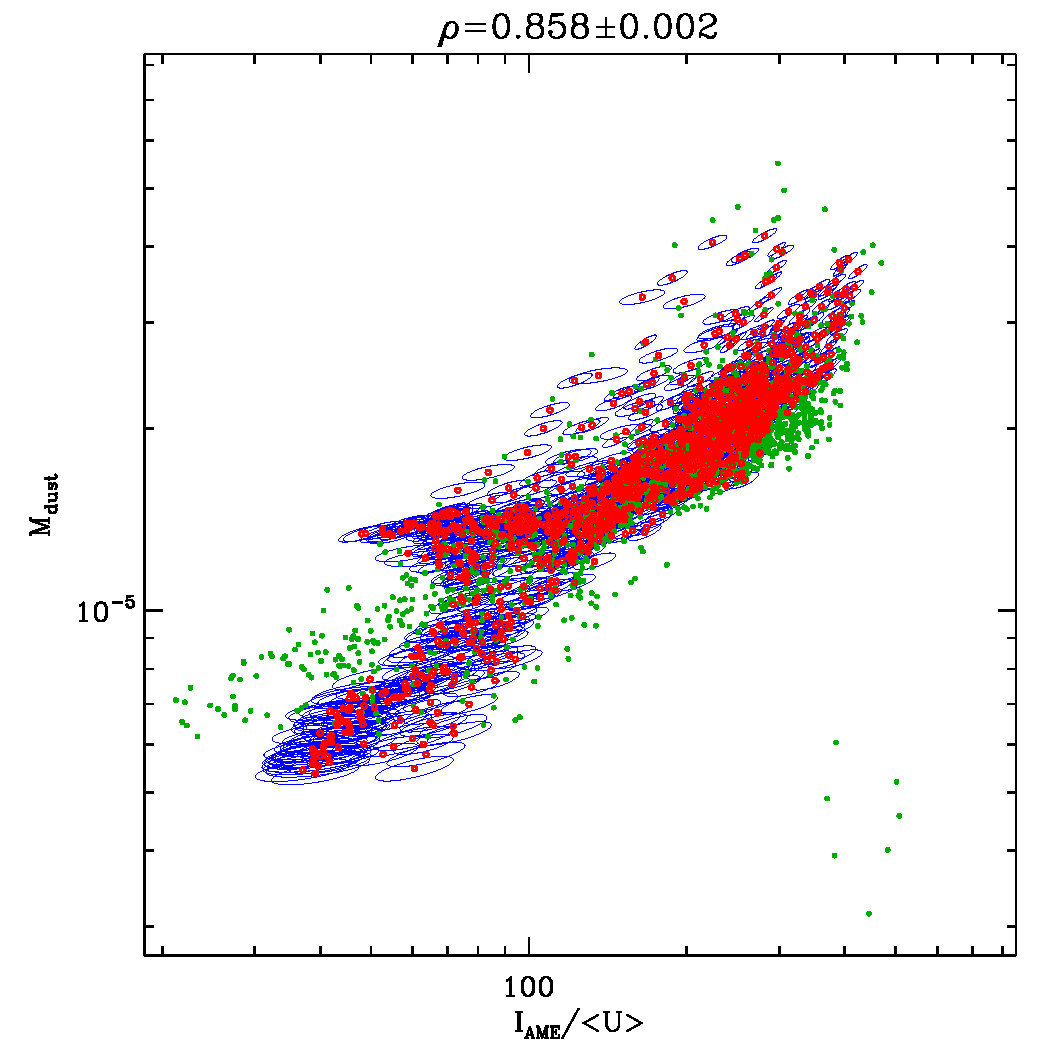
\includegraphics[width=\textwidth]{../Plots/ch_lori/corr_IameUav_lnMd.pdf}
                 \centering
                 \caption{Scatter plot with the bivariate error elipses generated through the \acrshort{hb} \acrshort{sed} fitting, of total dust mass $M_{dust}$ vs. $I_{AME}$ scaled by $U$. Green dots indicate the results when using a simple least-squares method fit, for comparison with the HB method.}
                 \label{fig:corr_IameUav_lnMd}
               \end{figure}
           \acrshort{ame} intensity is scaled by the \acrshort{isrf} intensity $U$. Although spinning dust emission is not predicted to vary directly with $U$, we consider that the ISRF may serve as a diagnostic of environmental conditions in the \acrshort{ism}. In any case, we find that performing such a scaling improves the correlations with dust mass.   Figs.~\ref{fig:corr_IameUav_lnMpah} and~\ref{fig:corr_IameUav_lnMpahion} describe the variation with $M_{PAH}$ and $M_{PAH+}$.
              \begin{figure}
                \includegraphics[width=\textwidth]{../Plots/ch_lori/corr_IameUav_lnMpah.pdf}
                \centering
                \caption{The same comparison is given by~\ref{fig:corr_IameUav_lnMd}, but showing total mass of \acrshort{pah}s ($M_{PAH}$) rather than total dust mass on the y-axis. }
                \label{fig:corr_IameUav_lnMpah}
              \end{figure}
              \begin{figure}
                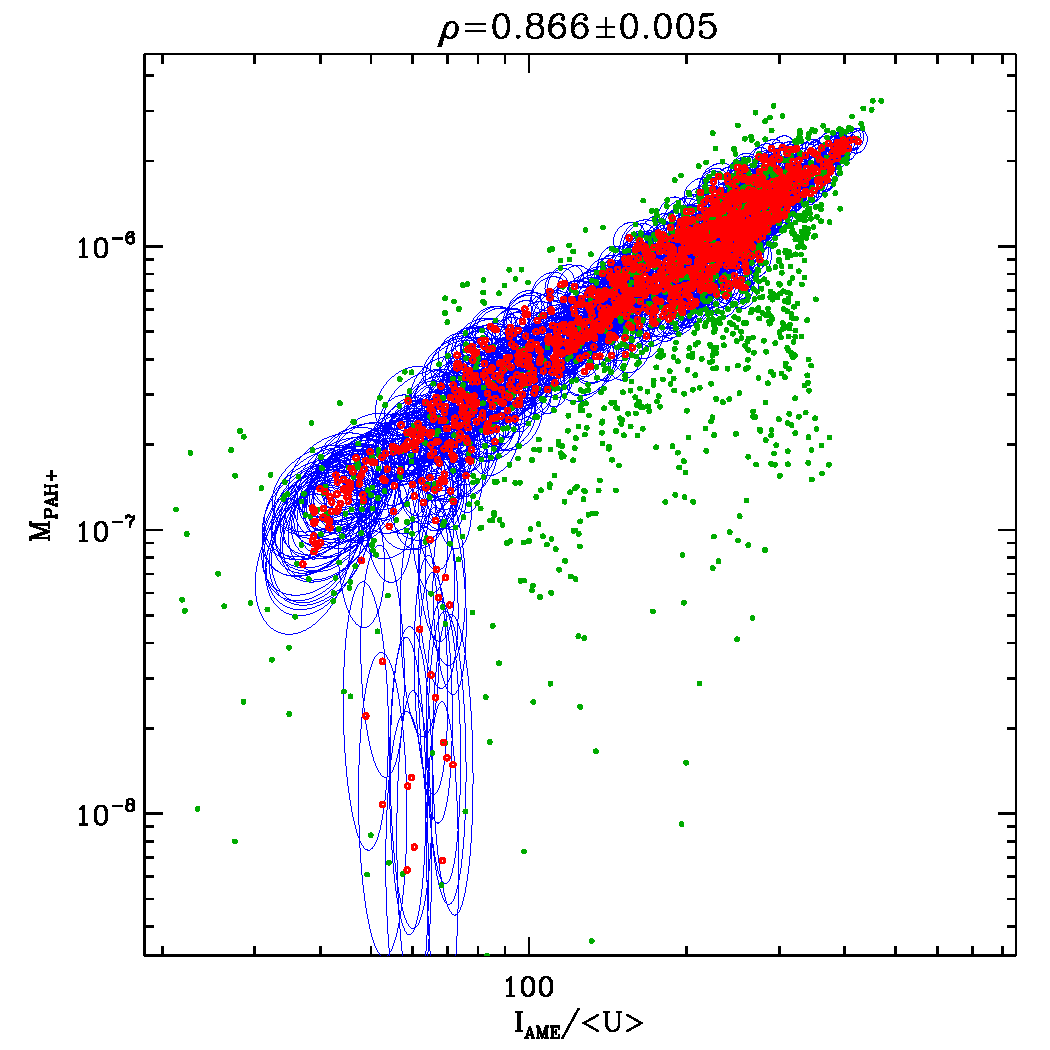
\includegraphics[width=\textwidth]{../Plots/ch_lori/corr_IameUav_lnMpahion.pdf}
                \centering
                \caption{ The same as in Figs.~\ref{fig:corr_IameUav_lnMd} and~\ref{fig:corr_IameUav_lnMpah}, but specifically comparing an estimate of the charged component of \acrshort{pah} mass $M_{PAH+}$. This includes anions and cations, since we cannot distinguish between these two spectroscopically.}
                \label{fig:corr_IameUav_lnMpahion}
              \end{figure}
    Based on the dust properties derived from these \acrshort{sed} fits, we investigate whether any fitted parameter shows a preferential relation with the \acrshort{ame}. Figs.~\ref{fig:corr_IameUav_lnMd}-\ref{fig:corr_IameUav_lnMpahion} reveal a very similar trend between the \acrshort{ame} and the parameters $M_{PAH}$, $M_{PAH+}$, and $M_{dust}$. There is a slightly improved correlation between $M_{dust}$ and $M_{PAH}$ (0.857 vs 0.867). This is consistent with the intensity cross correlations in Fig.~\ref{fig:orionis-corr-matrix}. These corrleations are discussed further in Sec.~\ref{sec:lori_discussion} and Fig.~\ref{fig:PDFs_Iame}.

    \subsection{Masking of the Central Region}
        To assess the effect of the morphology of $\lambda$~Orionis on the SED fitting results, we repeat the analysis with a mask applied to the central region. This allows us to focus on the variation of correlation strengths within the ring structure, which is less affected by heating from the $\lambda$Ori association. Fig.~\ref{fig:center_mask} indicates the mask applied. Fig.~\ref{fig:PDFs_center_masked_Iame}, in the same way as Fig.~\ref{fig:PDFs_Iame}, indicates the PDFs for the correlation scores of AME vs. dust mass, PAH mass, and ionized PAH masss--- but this time excluding pixels from the central portion of $\lambda$~Orionis.
        \begin{figure}
          \includegraphics[width=\textwidth]{../Plots/ch_lori/PDFs_center_masked_Iame.pdf}
          \centering
          \caption{ The hierarchical Bayesian correlation probablity distributions of $\rho{s}$) for the three physical parameters vs. the \acrshort{ame} intensity: total dust mass, $\rho_{dust}$ (red); total \acrshort{pah} mass $\rho_{PAH}$ (green); and only the ionized \acrshort{pah} mass $\rho_{PAH+}$ (blue). Also given are the probabilities of either \acrshort{pah} component being better correlated with \acrshort{ame} than dust mass, as well as the probability that ionized \acrshort{pah} mass correlates better than total \acrshort{pah}.}
          \label{fig:PDFs_Iame}
        \end{figure}

  \section{Discussion}
  \label{sec:lori_discussion}
      In  $\lambda$~Orionis we found that accross the whole region, A9 emission and P545 emission were the most strongly correlated with \acrshort{ame}. This is apparent both in the photometric band analysis, and in the dust \acrshort{sed} fitting.  The fact that the correlation strengths of \acrshort{pah}-tracing mission and sub-mm emission are similar is in-line with what we have seen in \cite{ysard10b} and \cite{hensley16}. In those works, the two relationships (\acrshort{mir} vs. \acrshort{ame} and \acrshort{fir} vs. \acrshort{ame}) are very close, although these two papers are odds as to which relationship is stronger, and thus in their final interpretation. With the present data and analysis of $\lambda$~Orionis, we fail to rule out \acrshort{pah}s as carriers of the \acrshort{ame}. Fig.~\ref{fig:PDFs_Iame} indicates that although total dust mass and \acrshort{pah} mass are both correlated with \acrshort{ame}, there is a strong (\textasciitilde{}100\%) probability that \acrshort{pah} mass is the stronger predictor of \acrshort{ame} intensity.
          \begin{figure}
            \includegraphics[width=\textwidth]{../Plots/ch_lori/PDFs_Iame.pdf}
            \centering
            \caption{ The hierarchical Bayesian correlation probablity distributions of $\rho{s}$) for the three physical parameters vs. the \acrshort{ame} intensity: total dust mass, $\rho_{dust}$ (red); total \acrshort{pah} mass $\rho_{PAH}$ (green); and only the ionized \acrshort{pah} mass $\rho_{PAH+}$ (blue). Also given are the probabilities of either \acrshort{pah} component being better correlated with \acrshort{ame} than dust mass, as well as the probability that ionized \acrshort{pah} mass correlates better than total \acrshort{pah}.}
            \label{fig:PDFs_Iame}
          \end{figure}
        The results are consistent with a scenario in which \acrshort{pah} mass, cold dust, and the \acrshort{ame} are all tightly correlated. A correlation between cold dust and \acrshort{pah}s is observed in extragalactic targets \citep{haas02}, and may be inferred from the correlation between \acrshort{uir} and \acrshort{fir} emission reported in diffuse galactic \acrshort{ism} \citep{onaka96}. In the case that \acrshort{ame} emanenates from spinning \acrshort{pah}s, it is not surprising that cold dust would also correlate with the \acrshort{ame}. Weaker correlation from 25 to 70~$\mu$m may indicate that \acrshort{ame} is weaker in regions of warmer dust and stronger radiation fields. Such an anti-correlation with harsher radiation are consistent with the carriers of \acrshort{ame} being destroyed in the central region of $\lambda$~Orionis, thus leading to substantially decreased spinning dust emission.

      \subsection{Performance of the Hierarchical Bayesian Fitting}

      Indicated in Figs.~\ref{fig:corr_IameUav_lnMd}, \ref{fig:corr_IameUav_lnMpah}, and\ref{fig:corr_IameUav_lnMpahion}, the trends described in this chapter between dust mass and \acrshort{pah} mass, and the \acrshort{ame} intensity were revealed through the \acrshort{hb} analysis. The increased scatter of best-fit points, produced by the least-squares analysis, obviously obscures the intrinsic relationships. With only \acrshort{lsm} results, the dust \acrshort{sed} fitting comparison would have been inconclusive. To our knowledge, this is the first case of the \acrshort{hb} approach being applied to a localized investigation of \acrshort{ame}, and certainly the first time that the dust \acrshort{sed} of $\lambda$~Orionis region has been investigated in such a way. This raises questions about the future of \acrshort{lsm}-based analysis in dust \acrshort{sed} studies, and highlights the potential this \acrshort{hb} framework developed by \cite{galliano18}.

      \subsection{PAH Ionization fraction}
          As described in Ch.\ref{ch:datasources} it is expected that relative variations between the A9 and I12 intensities could be explained by the fraction of \acrshort{pah}s that are charged, $fPAH+$. Spectroscopically, we cannot distinguish between \acrshort{pah} anions or cations. However if spinning dust emission arises from anions, a better correlation with the mass of charged \acrshort{pah}s $M_{PAH+}$ is expected. However if the \acrshort{pah}s are positively charged, a stronger correlation with $M_{PAH+}$ is not expected. This is due to the rotational excitability of the \acrshort{pah}s: anions are more succeptable to rotational excitation by $H^{+}$ and $C^{+}$ collisions\citep{ali-haimoud10}.

          Examining $\lambda$~Orionis in intensity, we find that the A9 intensity correlates more strongly with \acrshort{ame} than I12 or D12. In the $r_{p}$ case, A9 correlates more strongly with \acrshort{ame} than any other band. This is consistent with the spinning \acrshort{pah} hypothesis, and taken alone may indicate that the 6.2~$\mu$m feature emission from charged \acrshort{pah}s, may be a better predictor of \acrshort{ame} intensity.

          As shown by the dust \acrshort{sed} fitting however, the probability distributions (Fig.~\ref{fig:PDFs_Iame}) of $r_{p}(M_{PAH+}:I_{AME})$ do not indicate that ionized \acrshort{pah} mass correlates better with the total \acrshort{pah} mass. Attempts to estimate the $M_{PAH+}$ based on the available data appear to only add noise relative to $r_{p}(M_{PAH}:I_{AME})$. The means of the two distrubtions $r_{p}(M_{PAH+}:I_{AME})$  and $r_{p}(M_{PAH}:I_{AME})$ are similar and $r_{p}(M_{PAH+}:I_{AME})$ shows a wider distribution. Thus the question of whether or not \acrshort{ame} comes predominantly from charged \acrshort{pah}s remains open.

          The fact that A9 correlates more strongly than the 12~$\mu$m bands, at least suggests that this topic is worth further investigation. What is clear from the \acrshort{mir} and \acrshort{ame} morphology however, is that there is a transition from a relatively \acrshort{pah} depleted, warmer, stronger \acrshort{isrf} in the centerand warm dust in the center to a \acrshort{pah}-supporting region in the ring. Along this transition, there must be a decreasing radiation field with distance from dimnant heating sources, in $\lambda$~Orionis association. \cite{andrews16} predict a transition of \acrshort{pah} species along such a radiation field gradient, from complete \acrshort{pah} destruction in harsh environments, to survival of (sufficiently large) \acrshort{pah} anions near the surface of molecular clouds. Thus if our stronger correlation with A9 indicates charged \acrshort{pah}s, this could be consistent with \acrshort{pah} anions surviving in the portions of $\lambda$~Orionis which are emitting the strongest \acrshort{ame}. Future wide-area spectral mapping of the ${\lambda}$~Orionis region may be able to conclusively test for increased $fPAH+$ in regions with stronger \acrshort{ame}. This would also help us to understand the extent to which [NeII] emission may contribute to the I12 emission, and if this may lead to a relatively improved correlation between \acrshort{ame} and A9. Such studies would be strongly aided by higher resolution probing of spatial variations the \acrshort{ame} spectral profile.

\chapter{All-sky Analysis}
  \label{sec:analysis}
    What we present here is a test of the generalizability of results from Ch.\ref{ch:lori}, which focused on a particular structure on the sky, $\lambda$~Orionis.
    We first would like to note that ``all-sky analysis'' can be a bit misleading. The term tends to lead readers to the idea of a definitive study, answering a particular question for any given position on the sky.  While a truly all-sky analysis would be ideal, signal-to-noise constraints (mainly at high galactic latitudes), as well as confusion along the line of sight (mainly in the galactic plane), make a uniformly powerful study of the whole sky very challenging. Here we will indeed show results for the entire sky as a benchmark analysis, but for the core analysis we must mask certain regions dominated by systematic effects in order minimize biases for particular wavelenghts.

\section{Resolution matching}
    \subsubsection{Smoothing}
        As in Ch.~\ref{ch:lori}, this approach applies to a spatial resolution of approximately ~1$^{\circ}$. The resolution limimtation is imposed by the PC microwave component maps, which list an `effective resolution' of 60$'$ \citep{planck15X}. Thus we must apply a smoothing to most of our input datasets, which have native resolutions of a much finer scale (see Tab.~\ref{tab:data}), and Fig.~\ref{fig:AME_contours}. The data also come in a wide range of beam shapes with their own degrees of uncertainty, thus we conservatively smooth all of the data in the same way, using a circular Gaussian beam, to have ~1$^{\circ}$ FWHM resolution. we ar We start with an all-sky AME to IR comparison, looking for global patterns among all pixels.

    \subsubsection{Offset correction}
      The most recent version of the pre-release full-sky IRC data contained an apparent all-sky positive offset of \~2~MJy/sr for A9 and \~4~MJy/sr for A18. We assess this offset first by finding the mode of each of the \~4,700 3x3 degree tiles of the IRC survey, and then taking the median of this distribution. We then compare this result with a monopole offset fit to the all-sky HEALPix map of the IRC surveys, built from these tiles. Monopole fitting is handled by the {\tt healpy.fit\_monopole} function. We find the values produced by these to methods to be consistent. We found offsets also in the IRAS, FIS, and HFI bands, thus we apply the same monopole fitting and subtraction to all of the all-sky maps. We do not find the correlation analysis presented in later sections to be sensitive to this offset correction.

  \section{All-sky cross correlations}
        In order to look more closely how the the AME to IR relationship varies with wavelength, we first do a comparison without applying any pixel mask, as a benchmark. Fig.~\ref{fig:AMEvsDust_allsky_allbands_mpsub_kde_unmasked} shows the pizel-density plots of AME vs. the IR bands' intensities. Darker regions show higher pixel densities, unshaded or more lightly shaded regions show low or zero pixel densities. An intial analysis, considering only the interreations of the PC parameter maps, was presented in Sec.~\ref{sec:PCmaps}, wherein correlations between the major microwave component maps (synchrotron, free-free, AME, and dust emisison) are demonstrated (Fig.~\ref{fig:PCCS_corrmatrix}). This section extends that analysis, considering the full range of IR maps described in Tab.~\ref{tab:data}. We see immediately that each band shows evidence of a positive trend with AME intensity. For the MIR bands, at lower IR intensities we see the effects of detector noise become dominant, turning into a more defined positive trend with increasing IR intensity. This effect is less pronounced in the FIR. The trend is similar to that found in Ch.~\ref{ch:lori}, and Fig.~\ref{fig:orionis-corr-matrix}.
          \begin{figure}
            \includegraphics[width=\textwidth]{../Plots/ch_allsky/AMEvsDust_allsky_allbands_mpsub_kde_unmasked.pdf}
            \centering
            \caption{Point-density distributions of the log $AME_{var}$ intensity (Y-axis) vs. log IR bands' intensities. In this case no pixel mask is applied, in order to show overall trend of the full data-set. However a random sampling is used due to computational contraints. The plots show a random set of 20\% of the full-sky data. Darker shaded regions indicate a higher density of pixels.}
            \label{fig:AMEvsDust_allsky_allbands_mpsub_kde_unmasked}
          \end{figure}
        We consider that the IR maps used must not only be compared to the AME, but to each other, to assess multi-wavelength patterns. We also compare the AME and IR maps to ancilliary maps, as decribed in Ch.~\ref{ch:datasources} and Tab.~\ref{tab:ancilliarydata}. Fig.~\ref{fig:all_bands_corr_matrix_wAME_spearman} confirms the weaker trend in the MIR vs. AME, via a cross-correlation matrix, similar to that used in Ch.~\ref{ch:lori} and Fig.~\ref{fig:orionis-corr-matrix}.
          \begin{figure}
            \includegraphics[width=\textwidth]{../Plots/ch_allsky/all_bands_corr_matrix_wAME_spearmanintensity_unmasked.pdf}
            \centering
            \caption{ALL-SKY cross-correlation matrix for the 12 infrared bands sampled, as well as the PC component maps described in Ch.~\ref{ch:datasources}: the two AME components evaluated at their peak frequencies $AME_{var}$, $AME_{fix}$; Syncrotron, and free-free), and ancilliary maps of $N_{H}$, $H_{\alpha{}}$ emission, and 408~MHz emission \cite{haslam82}. The color-scale indicates ($r_{S}$). Results are based on the unmasked sky, but are split by Galaxctic latitude: pixels with $|\beta{}| < 15deg$ (left) and $|\beta{}| > 15deg$ (right). The color and annotations indicate $r_{s}$ as in Fig.~\ref{fig:orionis-corr-matrix}. }
            \label{fig:all_bands_corr_matrix_wAME_spearman}
          \end{figure}
       This is reflected in the comparison between high and low latitude plots: for pixels $|\beta| > 15 deg$, we see a dramatic effect. In the most extreme case $r_{s}$ of A18 to $AME_{var}$ drops from 0.72 at lower latitudes, to 0.02 at higher latitudes. $r_{s}(A9:AME_{var})$ drops from 0.79 to 0.42. Correlations between the MIR bands and FIR bands also weaken. Only the the interrelations between the FIR bands from I60 to P545 remain eseentially latitude independent (with the exception of A65, which has an especially high noise level.)

        In the lower latitudes, with $|\beta| < 15deg$, bright emission in and around the galactic plane seems to homogenize the bands. We see little change from band to band both in terms of the relationship with AME or with other IR bands. Thus the increase of S/N with decreasing brightness at higher latitudes has a strong effect on such intensity correlation tests. Bands tracing bright thermal dust emission at higher latitudes are more robust against this effect. The only case where the trend is reversed, is with the maps of $N(H)$ and $H_{\alpha}$. Both of these maps show higher $r_{s}$ when compared to high latitude FIR emission. The next section descibes a pixel-masking strategy designed to mitigate both $r_{s}$ suppressing effects from band-to-band S/N variations, and $r_{s}$ enhancing effects from confusion near the galactic plane.

      \section{Masked Comparison}
        For the reasons described in the previous section, we consider that an exhaustive comparsion of the AME with IR requires the use of a pixel mask. In this section we describe the various masks applied to the full dataset. We then repeat both the comparisons above (as in  Figs.~\ref{fig:AMEvsDust_allsky_allbands_mpsub_kde_unmasked} and~\ref{fig:all_bands_corr_matrix_wAME_spearman}) for the masked dataset, and present additional analyses. The full mask, applied to the A9 map, is shown in Fig.~\ref{fig:A9_masked_map}.
          \begin{figure}
            \includegraphics[width=\textwidth]{../Plots/ch_allsky/masked_map_A9.pdf}
            \centering
            \caption{All-sky map in A9 emission after applying the combined masks: ecliptic plane, galactic plane, point sources, and pixels with S/N $<3$. This mask essentially outlines the galaxy, except for the most confused regions. Diffuse galactic emission is essentially removed by the mask due to low S/N in the MIR bands. In the full sky map of \~700,000 pixels, there are ~50,000 unmasked pixels remaining.}
            \label{fig:A9_masked_map}
          \end{figure}

      \subsection{Pixel mask}
          We prepare a global pixel mask (pixel positions masked in any map are excluded from the analysis).

        \paragraph{Galactic plane}
          The galactic plane tends to be a challenge in any comparison, but especially with low resolutions studies such as the present work. Complicated structures along the line of sight, smoothed to 1 degree resolution, means that emisison within any given pixel is an average of many different environments (evidenced by the homogenizing of the correlations between bands at low latitudes in Fig.~\ref{fig:all_bands_corr_matrix_wAME_spearman}.) Thus we exclude the brightest emission of the galactic plane, according to the mask prepared by the Planck Collaboration.

        \paragraph{Zodical light}
          To keep our analysis comparable to previous works, we exclude pixels within 10$^{\circ}$ of the ecliptic plane \citep{hensley16}.  Even though we use the Zodi-subtracted maps \citep{kelsall98, kondo16, ootsubo16}, the Zodi residuals are still problematic (especially in the MIR.) This corresponds to regions with the heaviest contamination from Zodiacal light, where Zodi residuals are apparent even with visual inspection for all of the MIR bands used in this study. In Ch.~\ref{ch:datasources}, Figs. \ref{fig:ratioMap_A9I12}, and \ref{fig:ratioMap_A9I12} clearly display these residual patterns.

        \paragraph{Signal to noise}
          Some of the bands used lack sufficient sensitivity to trace fainter emisison, especially at higher galactic latitudes. This is mainly an issue for the mid-infrared bands. As such, we enforce a $3~\sigma$ threshold for all of the maps--- adding to the mask any pixel that has lower than $~\sigma$ detection in any of the maps. This removes nearly all pixels beyond approx. 15 degrees from the galactic plane, with the pronounced exception of regions affected by stray moonlight. The extent of this particular mask is primarily defined by the IRC A9 and A18 maps, which have the highest noise levels.

        \paragraph{PC Component Separation Errors}
          As noted in \cite{planck15X, hensley16} and displayed in Fig~\ref{fig:R_PCAMEtoPCdust}, there are fluctuations in the PC maps wherein AME emission appears to correspond to fluctuations in the synchrotron or free-free component maps.

       \paragraph{Point Sources}
         The Planck Collaboration provides masks of the pixels they find to include point sources. We mask pixels which are flagged as being point-source contaminated, in the most heavily affected maps: Planck/HFI~857 GHz and Planck/LFI~30 GHz.
           Fig.~\ref{fig:AMEvsDust_allsky_allbands_mpsub_kde_masked} shows point-density plots for $AME_{var}$ vs. each of the IR bands, after applying the mask described above.
              \begin{figure}
                \includegraphics[width=\textwidth]{../Plots/ch_allsky/AMEvsDust_allsky_allbands_mpsub_kde_masked.pdf}
                \centering
                \caption{The same comparison as shown for Fig.~\ref{fig:AMEvsDust_allsky_allbands_mpsub_kde_unmasked}, but with the mask applied as in Fig.~\ref{fig:A9_masked_map}.}
                \label{fig:AMEvsDust_allsky_allbands_mpsub_kde_masked}
              \end{figure}
            As expected with such a drastic reduction of the number of noise-dominated points, the scatter, especially for the MIR bands, is reduced. Otherwise the applicaiton of the mask does not bring about any special distinction among the bands when compared to the AME. What is notable however is that the persistent weakening of trend of I25 vs. AME, relative to A9 and the FIR bands. Following the logic that the PAH-tracing bands intensity is essentially a product of the ISRF ($U$) and the column density of PAHs ($\sigma_{PAH}$), we redraw the comparison after scaling the IR bands by $U$. We do this not only for the MIR bands, simply for comparison. We do not have a theoretical prediction as to the relationship between AME intensity and the FIR bands' intensities scaled by $U$. The pixel density plots for such a comparison are given by Fig.~\ref{fig:AMEvsDust_allsky_allbands_mpsub_UNorm_kde_masked}, which is the same as Fig.~\ref{fig:AMEvsDust_allsky_allbands_mpsub_kde_masked} except for division of the X-axes by $U$.
              \begin{figure}
                \includegraphics[width=\textwidth]{../Plots/ch_allsky/AMEvsDust_allsky_allbands_mpsub_UNorm_kde_masked.pdf}
                \centering
                \caption{Similar comparison to Fig.~\ref{fig:AMEvsDust_allsky_allbands_mpsub_kde_unmasked}, with the IR intensities scaled by $U$ for each pixel. }
                \label{fig:AMEvsDust_allsky_allbands_mpsub_UNorm_kde_masked}
              \end{figure}
            Corresponding to the plots vs. AME given in Figs. Fig.~\ref{fig:AMEvsDust_allsky_allbands_mpsub_UNorm_kde_masked} and~\ref{fig:AMEvsDust_allsky_allbands_mpsub_kde_masked}, we again perform a cross-correlation matrix test, to understand how the bands relate to one another- not only to the AME. This cross-correlation is done for both intensity, shown by Fig.~\ref{fig:all_bands_corr_matrix_wAME_spearmanintensity_maskall} and $U$ normalized intensities showin in Fig.~\ref{fig:all_bands_corr_matrix_wAME_spearmanU_norm_masked}.
              \begin{figure}
                \includegraphics[width=\textwidth]{../Plots/ch_allsky/all_bands_corr_matrix_wAME_spearmanintensity_maskall.pdf}
                \centering
                \caption{Cross-correlation ($r_{s}$ matrix for the IR intensities (unscaled) vs. each other, esssentially the same comparison as in Fig.~\ref{fig:all_bands_corr_matrix_wAME_spearman}, except that the pixel mask is applied.}
                \label{fig:all_bands_corr_matrix_wAME_spearmanintensity_maskall}
              \end{figure}
              \begin{figure}
                \includegraphics[width=\textwidth]{../Plots/ch_allsky/all_bands_corr_matrix_wAME_spearmanU_norm_masked.pdf}
                \centering
                \caption{Cross-correlation ($r_{s}$ matrix for the $U$-normalized IR intensities vs. each other, and also against the AME components, other PC products, and ancilliary data. Only the IR maps are divided by $U$- other data is unchanged from Fig.~\ref{fig:all_bands_corr_matrix_wAME_spearmanintensity_maskall})}
                \label{fig:all_bands_corr_matrix_wAME_spearmanU_norm_masked}
              \end{figure}

          \paragraph{Bootstrap test}
              In addition, for the masked comparison, we carry out a boostrap analysis similar to that discussed in Ch.~\ref{ch:lori} and Fig.~\ref{fig:bootstrap_vs_AME}. The Spearman rank correlation coefficents $r_{S}$ of all of the bands, in intensity, vs. the $AME{var}$ component are shown. This is done only for the masked case, due to the computational challeneges presented by a well-sampled bootstrap of all \~780,000 pixels in the full sky. Because the mask applied here leaves us with approximately 1/7 of the sky, a bootstrap with $N_{iterations} > N_{pix}$ becomes tractable. We show the comparison only for the $AME_{sum}$ component also due to computational constraints. The $r_{s}$ distributions for each IR band vs. AME are shown in Fig.~\ref{fig:bootstrap_vs_AME_allsky_masked}.
                \begin{figure}
                     \includegraphics[width=\textwidth]{../Plots/ch_allsky/bootstrap_vs_AME_spearman_maskall_i1000.pdf}
                     \centering
                     \caption{.}
                     \label{fig:bootstrap_vs_AME_allsky_masked}
                \end{figure}

\section{Spatial variaton of correlations}
    To understand how these trends may vary across the sky, we produce an all-sky maps of $r_{s}$ for AME vs. IR emission, without employing any pixel mask. From the NSIDE~256 input maps of AME and 4 IR wavelength maps, we produce NSIDE~8 maps of $r_{s}$. These maps are shown in Figs.~\ref{fig:Spearman_Map_nside8_AMEtoIR_A9} and~\ref{fig:Spearman_Map_nside8_AMEtoIR_I12}.
      \begin{figure}
        \includegraphics[width=\textwidth]{../Plots/Allsky_Corr/Spearman_Map_nside8_A9toAMEvar.pdf}
        \centering
        \caption{Spatial map of $r_{s}$ between the AME and IR intensity for 4 bands:$9~\mu{}m$, $12~\mu{}m$, $25~\mu{}m$, and $140~\mu{}m$. $r_{s}$ is calculated for all NSIDE~256 pixels within each NSIDE~8 pixel-sized bin.}
        \label{fig:Spearman_Map_nside8_AMEtoIR_A9}
      \end{figure}
      \begin{figure}
        \includegraphics[width=\textwidth]{../Plots/Allsky_Corr/Spearman_Map_nside8_I12toAMEvar.pdf}
        \centering
        \caption{}
        \label{fig:Spearman_Map_nside8_AMEtoIR_I12}
      \end{figure}
      \begin{figure}
        \includegraphics[width=\textwidth]{../Plots/Allsky_Corr/Spearman_Map_nside8_I25toAMEvar.pdf}
        \centering
        \caption{}
        \label{fig:Spearman_Map_nside8_AMEtoIR_I25}
      \end{figure}
      \begin{figure}
        \includegraphics[width=\textwidth]{../Plots/Allsky_Corr/Spearman_Map_nside8_A140toAMEvar.pdf}
        \centering
        \caption{}
        \label{fig:Spearman_Map_nside8_AMEtoIR_A140}
      \end{figure}

     \begin{figure}
       \includegraphics[width=\textwidth]{../Plots/Allsky_Corr/RadNorm/Spearman_Map_nside8_AMEtoA9.pdf}
       \centering
       \caption{Spatial map of $r_{s}$ between the AME and IR intensity as in Fig.~\ref{fig:Spearman_Map_nside8_AMEtoIR_A9}, but with the AME and IR maps first normalized by dust radiance $R$.}
       \label{fig:Spearman_Map_nside8_AMEtoIR_radnorm_A9}
      \end{figure}
       \begin{figure}
        \includegraphics[width=\textwidth]{../Plots/Allsky_Corr/RadNorm/Spearman_Map_nside8_AMEtoI12.pdf}
        \centering
        \caption{}
        \label{fig:Spearman_Map_nside8_AMEtoIR_radnorm_I12}
      \end{figure}
        \begin{figure}
         \includegraphics[width=\textwidth]{../Plots/Allsky_Corr/RadNorm/Spearman_Map_nside8_AMEtoI25.pdf}
         \centering
         \caption{}
         \label{fig:Spearman_Map_nside8_AMEtoIR_radnorm_I25}
      \end{figure}
        \begin{figure}
        \includegraphics[width=\textwidth]{../Plots/Allsky_Corr/RadNorm/Spearman_Map_nside8_AMEtoA140.pdf}
        \centering
        \caption{}
        \label{fig:Spearman_Map_nside8_AMEtoIR_radnorm_A140}
        \end{figure}


    \section{Discussion}
      \subsection{AME:Dust}
        As noted in Ch. \hyperref[ch:intro]{\ref{ch:intro}}, previous studies found that the AME generally correlates at dust-related IR wavelengths \citep{ysard10b,planckXV, hensley16}. We see the same overall pattern in the present study.

         In our all-sky comparison, we find a first-order correlation between IR intensity and AME intensity, for each of the 12 wavelengths sampled. This is again consistent with the previous investigations of the AME cited above, in that the FIR emission shows the tightest correlation with the AME intensity.

         In testing for a second-order correlation, we divided the IR intensities and AME intensity by the dust radiance, and again performed the band-by-band all-sky comparison. There is evidence of a residual correlation between $I_{MIR}$ and $I_{AME}/R$. Unsurprisingly, the strong correlation between $I_{FIR}$ and $I_{AME}$ disappears when scaling by $R$, as the the FIR bands are dominated by thermal dust emission. In this case, we again find no evidence of an improved correlation for the PAH-dominated bands.

           The closeness of the correlation coefficients found here is consistent with the results of the IRAS vs. AME correlation test result from \cite{planckXV}. They found that the correlation coefficient among the 4 IRAS bands (12, 25, 60, and 100~$\mu$m) differ from one another only by about 5\%, across the whole set of 98 regions. The trend of AKARI MIR and FIR data vs. the AME does not disagree with their IRAS comparison. This work adds that bands longer than IRAS 100~$\mu$m also correlate strongly with AME, especially the two Planck/HFI bands used.

          \subsection{AME:PAH}
            Each of the bands sampled show correlation with the AME, however the FIR bands always show the strongest correlation. In fact, the correlation pattern of AME vs. each of the IR bands, very strongly resembles the correlation results of the FIR vs. all of the other maps. This is readily apparent from the pixel-density plots in Figs.~\ref{fig:AMEvsDust_allsky_allbands_mpsub_kde_unmasked} and~\ref{fig:AMEvsDust_allsky_allbands_mpsub_kde_masked}, wherein the FIR bands pixels show a very similar density profile vs. the AME. In attempting to factor out this first-order correlation, dividing the AME and IR intensities by $U$ for each pixel, we find the there is still a residual correlation between the MIR bands and the AME.

          \subsection{AME:$T$, $G_{0}$}
            According to spinning dust theory outlined in \cite{draine98a} and in subsequent works by \cite{ysard10a}, the AME profile and intensity will depend in part on the ISRF- but as is well-stated in \cite{hensley17a}, exactly how the ISRF will affect the AME SED is a more complicated question. Absorbed starlight photons may be able to rotationally excite the carriers, but if an enhanced ISRF leads to increased dust heating, then the increased IR emission can rotationally de-excite the carriers. Moreover the ISRF affects not only the dust temperature but ionization of the carriers.

            %\cite{hensley16} looked at the $AME$/$R$ ratio vs. $T$ and found only a slight anti-correlation of $P = -0.06$.

          \subsection{Microwave foreground component separation}

            There are known degeneracies between the foreground parameters of the COMMANDER maps (spinning-dust, and free-free, synchrotron components as described in \cite{planck15X}.) This can be demonstrated by comparing the ratio map of the PCXV intensity to thermal dust intensity.

\chapter{Summary}
  \label{ch:Summary}

  In Ch.~\ref{ch:intro} we demonstrated the both the mysteries and potential for answers revealed by all-sky observation and analysis. A paticular mystery, that of the Anomalous Microwave Emission, and the popular but yet unproven hypothesis that this AME comes from rapidly spinning tiny dust grains, perhaps PAHs, was introduced. We explained the merit of testing a spinning PAH hypothesis, while noting that spinning nanosilicates, or even magnetic dipole emission from dust have also been put forth in the literature.

  In Ch.~\ref{ch:datasources}, we overviewed a collection of infrared all-sky surveys that help us prove the dust SED from the UIR band range to the FIR, and discussed how these could help explore the AME question. We described also complimentary data and parameter maps from the Planck Collaboration that can be compared with the IR maps. Particular advantages of the PAH tracing bands, especially the A9 band, for covering not only neutral but potentially charged PAHs, were discussed in the context of AME investigation. Limitations were given for all of these data sets--- most of these boiling-down to component separation either of the Zodical light from thermal dust emission, or to the latter from other microwave foregrounds and the CMB.

  In Ch.~\ref{ch:lori} we combined and processed the data presented in Ch~\ref{ch:datasources} to investigate a particular region of the sky with relatively high S/N in all of the data, and demonstrating strong AME. We evaluated the background, noise, and contamination from systematic errors and point sources in these data, and compared them on a common resolution and grid. All of the analyses from simple correlation plots, to bootstrap analysis, to dust SED fitting suggest that A9 emisison correlates with AME better than I12 or D12- supporting PAH emisison as the source of AME, and suggesting the role of charged PAHs should be further explored. In addition we find that the bands near the thermal dust emisison peak show a weaker correlation, perhaps suggesting that harsh radiation fields may be destroying PAHs, leading to weaker AME. We also cautioned that although PAH mass correlates better than dust mass, we still see a good correlation between FIR emisison and AME (P545, P857). This raises the possibility that AME, PAHs, and cold dust are all correlated.

  In Ch.~\ref{ch:allsky} we attempted to find evidence that the result from Ch.~\ref{ch:datasources} applies even when looking at a less region-specific scale, using an all-sky analysis. However neither the full-sky unmasked case, or the case employing a mask of low S/N regions (mainly high galactic latitudes), point sources, and the galactic plane, showed a stronger correlation between PAH related emission and AME than that seen between FIR emission and the AME. We did however find that as in Ch.~\ref{ch:lori}, A9 tends to correlate with AME better than I12 or D12. We discussed apparent systemtic issues with the AME data, such as the possibility for under or over subtraction of free-free or synchrotron emission, and how these could serve to weaken evidence of any PAH or small grain correlation wiht the AME. Scaling the infrared intensities by $U$ does not change this result. We reproduce the result from \cite{hensley16} that there is not an overall correlation between PAH fraction and AME-per-dust-emisison, but expand this calculation showing that for a few limited regions on the sky there may be evidence of a correlation. We discuss how a potential variation on the optical thickness between UIR bands, FIR emisison, among other factors, could lead do a different result between $\lambda$~Orionis and the all-sky analysis. We also discuss potential observional advances that could help explore the issue further.

  Overall, using the presently available data, it is difficult to isolate the PAH-dust relationship, from the dust-AME relationship. We find throughout this work that a PAH-emission to AME correlation is readily demonstable, in intensity. A test of whether a second-order relationship exists, such that PAH emission is a better predictor of the AME than thermal dust emission, was shown to be inconclusive. One exception is that of $\lambda$~Orionis, where our results suggest that PAH mass correlates better with AME than does the total dust mass. Nevertheless we emphasize this point cautiously, because we were not able to generalize it to a larger scale (all-sky data with, effectively, a mask on the galactic plane and high latitude emission.)  We are not able to confirm or reject a ``spinning PAH'' hypothesis for the source of AME. However in $\lambda$~Orionis, and perhaps other regions yet to be examined in with dust SED fitting, we suggest that there is still ample reason to continue testing this hypothesis.



%%%%%% appendix %%%%%%%
\appendix
\chapter*{A Note on Data Dimensionality}

While we aim to demonstrate the application of high dimensionality in these studies, we do not wish to mislead readers that we have assembled a 12-dimensional photometric dataset, simply because we have 12 wavebands. This statement may seem nonsensical at first, but makes sense when we consider the covariance of the data. Just from the outside, and our faithful belief that FIR dust emission looks something like a blackbody, or modified blackbody, or at the very least we can agree that emission from dust in thermal equilibrium would produce some sort of peaked continuum emission spanning multiple photometraic bands' width. If we agree on this point, then it follows naturally that said bands would be highly correlated with one another. This means that the number of truly independent data dimensions is not only lower than the number of bands used here, it is much lower.

Fig.~\ref{fig:pca_intro} shows the \% of variance in the data retained by the first $n$ principal components. Principal components are found essentially by first finding the covariance matrix of the input data, and then diaganolizing this matrix- the eigenvectors will be the basis vectors of each principal component. The eigenvalues will give the explained covariance per component. Applied in this manner, the components may not necessarily have a clear physical interpretation, but from a data analytics perspective we can at least assess the redundancies in our data. Thus from Fig.~\ref{fig:pca_intro}, and choosing an arbitrary covariance ``acceptable loss'' of 99\%, our photometric data set steeply reduces to 3 dimensions. The first component contains 98\% of the total variance.


\begin{figure}
  \includegraphics[width=\textwidth]{../Plots/ch_intro/pca_intro.pdf}
  \centering
  \caption{Explained variance decline for principal component analysis performed on a set of 12 all-sky infrared maps. The first three components account for over 99\% of the total variance. The PCA fit is performed on the whole sky, after whitening the data, using the ``scikitlearn }
  \label{fig:pca_intro}
\end{figure}


\singlespacing
\chapter*{Acknowledgements}
\addcontentsline{toc}{chapter}{Acknowledgements}
     I would like to thank Professor Takashi Onaka firstly for guiding me since I first came to his laboratory as an undergraduate summer intern, in June 2012. I'm not sure if I've worked hard enough for the honor of being his last Ph.D. student, but its been a pleasure. I am extremely happy that I to complete my degree here. I wish him the happies of retirements, while sincerely doubting he will be able to stay away from research for long.

     Onaka-sensei and the members of the Onaka-lab have literally helped me to survive here, assisting any time that I have had difficulty adjusting as a foreign student.

    Itsuki Sakon has helped me greatly from the moment I arrived in Japan (literally.) It is also quite refreshing when his driving skills leave me at my destination much earlier than planned.

     I have been very lucky to have helpful co-authors for the various posters and abstracts I have presented in the course of this thesis: Ho-Gyu Lee, Daisuke Ishihara, Yasuo Doi, Ho-Gyu Lee, Mark Hammonds, Fumihiko Usui, Takafumi Ootsubo, Ryou Ohsawa, Tamami Okada, Hidehiro Kaneda --- especially, my international collaborators kind enough to host me over the years, Ronin Wu, Mridusmita Buragohain, Rupjyoti Gogoi, Frederic Galliano, Amit Pathak, Martin Giard, and Olivier Berne.

     My undergraduate advisor, Steven Gibson, deserves a special thanks for continued kind encouragement and research advice even now that I have graduated from WKU.

     Most personally, I must thank my mother, Catherine Marie Bell who has supported me more than seems possible for a single human being. The same goes to my younger siblings, Joseph, Emma, Caleb, and Noah who I have too few opportunities to help grow up. I thank also Deborah and Faithie (``Mama'') Guffy, who have been like aunt and gradnmother to us all.

     My day to day life in Japan has been brightened by partner of five years, Yuki Sugisawa \begin{CJK}{UTF8}{min}(杉澤友紀)\end{CJK}. His family too, who have been an unofficial host-family over the years, Chikako \begin{CJK}{UTF8}{min}(千賀子様),Hiromi (宏美様), Takeshi (剛様), and Chiri\end{CJK}. Even his grandmother Junko and grandfather Sadao Masuda \begin{CJK}{UTF8}{min}(桝田順子と定雄様)\end{CJK} have shown me much kindness during my visits to Osaka.

     A special note of thanks is owed to my friends who have inspired me and shared moral support, from back in the US, throughout my program: Alexandria Boswell, Hannah Kagan-Moore, Alexander Chen, George Johnson, Nicolas Tarantino, and John Max Wilson; as well as my classmates at U.Tokyo, Scarlet Elgueta, Jerome de Leon, Ryouta Kawamata, Takahiro Sudoh, Taku Okamura, John Livingston, Kyle Mede, Yuta Kato, and others.

     This project could not have found its way to any assemblance of completion without kind and insightful discussions with Nathalie Ysard, Alessandra Candian,  Chikako Yasui, Norita Kawanaka, Bruce Draine, Chris Tibbs, Francois Boulanger, Brandon Hensley, Clive Dickinson, Yasushi Suto, Othman Benomar, and Anthony Jones.

     The staff of GRID, Inc., especially Mehdi Shibahara and Ying-Ming Chen, helped guide my career choices and advance my knowledge of machine learning besides being the best lunch pals.

     I wish the best of luck to my kohais in Onaka-lab: Izumi Endo, Jin Zhang, Tomoyuki Kimura, Ayato Ikeuchi, and Mingie Jian in their continued studies and careers. I also want to express special thanks to the staff of the International Liaison Office, for advising me over the last five years, even since I was an undergraduate research internship student, in the UTRIP program of 2012.

     This project acknowledges a wide range of authors. I would like also to credit especially any of those whose names did not make it into the literature, for whatever reason. Especially the many women and minorities who have made direct or indirect contribtuions to science, but have been systematically overlooked and underrepresented in journals and awards.

     My financial support for living and tuition expenses during this time has been generously provided by "MEXT", the Ministry of Education, Culture, Sports, Science and Technology (\begin{CJK}{UTF8}{min}文部科学省.\end{CJK}). This research is based on observations with AKARI, a JAXA project with the participation of ESA; Planck (http://www.esa.int/Planck), an ESA science mission with instruments and contributions directly funded by ESA Member States, NASA, and Canada; and IRAS, a joint project of the US, UK and the Netherlands.

    This research made use of Montage. It is funded by the National Science Foundation under Grant Number ACI-1440620, and was previously funded by the National Aeronautics and Space Administration's Earth Science Technology Office, Computation Technologies Project, under Cooperative Agreement Number NCC5-626 between NASA and the California Institute of Technology


\small
\bibliographystyle{apj}
\bibliography{reference}
\end{document}
